% MARINA VON STEINKIRCH, SPRING/2013
% http://mysbfiles.stonybrook.edu/~mvonsteinkir/
\documentclass[11pt]{article}

\usepackage{epsfig}
\usepackage{color}
\usepackage{amsmath}    % Package  for subequations
\usepackage{graphicx}   % Package for figures
\usepackage{verbatim}   % Package  for program listings
\usepackage{hyperref}   % Package  for hypertext links, external documents and URLs
\usepackage{amssymb} % For mathematical constructions
\usepackage{latexsym} % Package to generate mathematical symbols
\usepackage{makeidx} % Package to generate an index in the end


\newcommand{\ie}{{\it i.e., }}
\newcommand{\eg}{{\it e.g., }}


\title{CSE 590: Computational Photography\\  Homework \#2: Image Blending }
\author{ \texttt{ Marina von Steinkirch, steinkirch@gmail.com}\\
	   \texttt{State University of New York at Stony Brook}}
\date{\today}




\begin{document}
\maketitle
\numberwithin{equation}{section}  




\section{Introduction}

This project explores the gradient-domain processing, a technique with many applications including:
\begin{itemize}
\item blending, 
\item tone-mapping, 
\item and non-photorealistic rendering.
\end{itemize}  

\quad

The  goal of this assignment is to {\it seamlessly blend} an object  from a source image into a target image. If we naively tried a simple cut and paste, we would see noticeable {\it seams}.  However, using the {\it Poisson blending technique} \cite{pois}, we are able  to achieve better results than just cutting and pasting.  The technique consists on finding values for the target pixels that {\it maximally preserve the gradient} of the source region, without changing any of the background pixels. In other words, we preserve the integrity of the gradient at the seams.

\quad 

The Poisson blending technique is solved as a {\it least squares problem}, \ie given the pixel intensities of the source image, $s$, and of the target image, $t$, we  solve for {\it new intensity values},  $v$, within the source region $S$:

\begin{equation}
v = \mbox{ argmin} \sum_{i \in S, j \in N_i, S} \Bigg ( \Big ( v_i -v_j\Big) - \Big (s_i - s_j \Big) \Bigg)^2 +  \sum_{i \in S, j \in N_i, -S} \Bigg ( \Big ( v_i -t_j\Big) - \Big (s_i - s_j \Big) \Bigg)^2. 
\label{aa}
\end{equation}

\quad

The idea is to recover an image that is best reflected by this edited gradient. Since the gradient provides us with linear constraints for every pixel in every color channel,
$$I_{i,j} - I_{i+1,j} = \frac{\partial}{\partial x},$$
and
$$I_{i,j} - I_{i,j+1} = \frac{\partial}{\partial y},$$
 we can formulate a {\it overdetermined system of linear equations}. Moreover, we set the desired {\it gradient field} $A x$ equals to the constraints defined by the vector field $b$ of the two images. The matrix $A$ can be seen as the representation of the gradient as a  {\it linear transformation} of the original image $x$. The result is a {\it large linear system} for each color channel with {\it one variable per pixel}, $Ax=b$. 

\quad

\section{Results}

\quad

\subsection*{Toy Model: Reconstruction of an Image from its Gradient}

We start by showing that an image can be reconstructed by its gradient values, where we:
\begin{itemize}
\item preserve x-y gradients, and
\item preserve intensity of one pixel.
\end{itemize}

\quad

For this objective, we denote the {\it intensity of the source image} at $(x, y)$ as $s(x,y)$ and the value to solve for as $v(x,y)$ and, for each pixel, we had three objectives: 
\begin{itemize}
\item minimize $\Bigg (v(x+1,y)-v(x,y)\Big) - \Big(s(x+1,y)-s(x,y)\Big) \Bigg)^2 $,
\item minimize $\Bigg( \Big(v(x,y+1)-v(x,y)\Big) - \Big(s(x,y+1)-s(x,y)\Big) \Bigg)^2 $, 
\item minimize $\Big(v(1,1)-s(1,1)\Big)^2 $, \ie adding any constant value to $v$.
\end{itemize}

\quad

Processing the sample image with this recipe return an identical image, with  {\it root square} equal to $2.3631\times 10^{-5}$.





\quad

\subsection*{Poisson Blending}

To solve the Poisson blending for two images, we implement the following steps:
\begin{enumerate}
\item we select source and target regions (Fig. \ref{1}-1 and  \ref{1}-2),
\item we get a mask for the source image, and align the two images and the mask (Fig. \ref{1}-3 and \ref{1}-4),
\item we solve the blending constraints described in the Eq. \ref{aa},
\item we copy the solved values into the target image, where for RGB images each channel is processed separately. The cut and past and the final blending results can be seen in the Fig. \ref{1}-5 and  \ref{1}-6.
\end{enumerate}

\quad

In the Figs. \ref{1}, we see that the Poisson blending worked nicely (no seams). This is due the fact that  the penguin is surrounded by snow in the source image, matching the snow in the background of the target image. We also notice that  the overall intensity of the penguin is darker with the Poisson blending technique. This is due the fact that the intensity of the surrounding snow is slightly darker in the target area.

\quad 

The same successful result can be see in the Fig. \ref{2}. The figures also  illustrate the noticeable seam in the naive cut and paste cropping.  In the other hand, in the Figs. \ref{3} and \ref{4} we see some failure examples of the Poisson blending. This is due the fact that the background of the two chosen images do not match even when taking the gradients.

\quad

\begin{figure} [ht]
\begin{center}
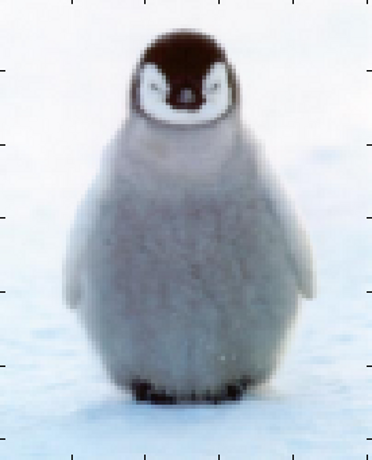
\includegraphics[scale=0.44]{results_poisson/set1/im1.png}  
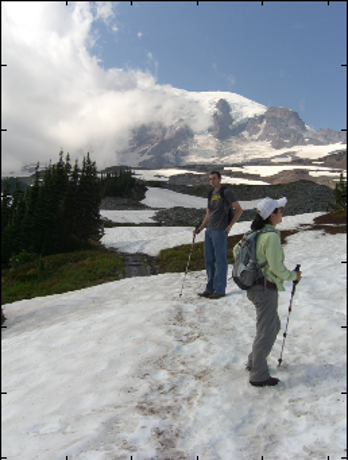
\includegraphics[scale=0.44]{results_poisson/set1/im2.png}
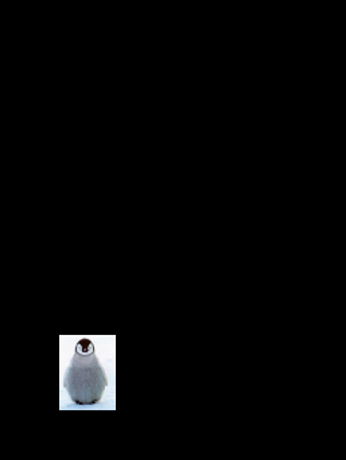
\includegraphics[scale=0.44]{results_poisson/set1/im3.png}  
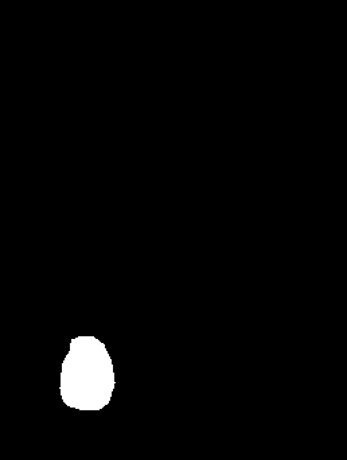
\includegraphics[scale=0.44]{results_poisson/set1/im4.png} 
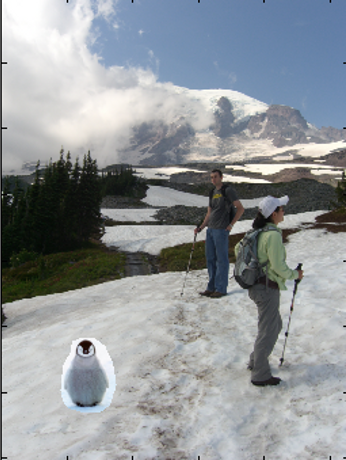
\includegraphics[scale=0.44]{results_poisson/set1/im5.png}  
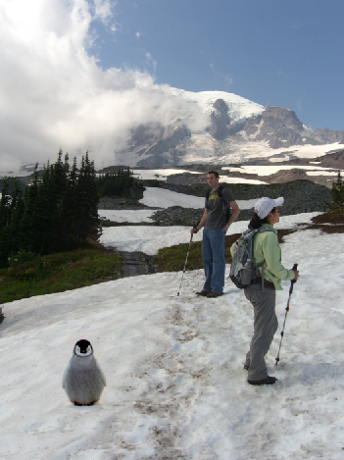
\includegraphics[scale=0.44]{results_poisson/set1/im6.png}   
\caption{Sample example of Poisson blending. (left, top) Source object, (middle, top) background image, (right, top) aligned source, (left, bottom) user input mask, (middle, bottom) cut and paste result, (right, bottom) Poisson blending final result.}
\label{1}
\end{center}
\end{figure}


\quad

\begin{figure} [ht]
\begin{center}
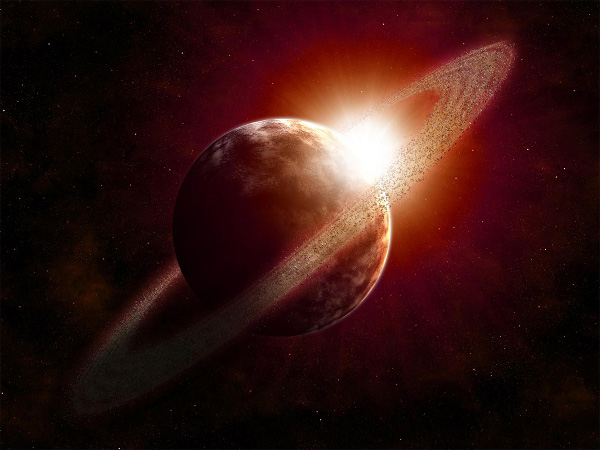
\includegraphics[scale=0.29]{results_poisson/set4/im1.jpg}  
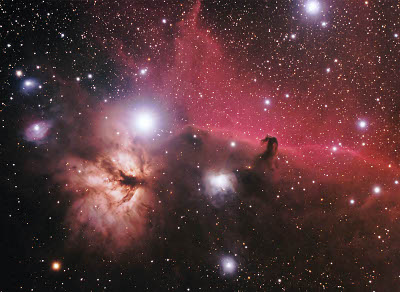
\includegraphics[scale=0.155]{results_poisson/set4/im2.jpg}\\
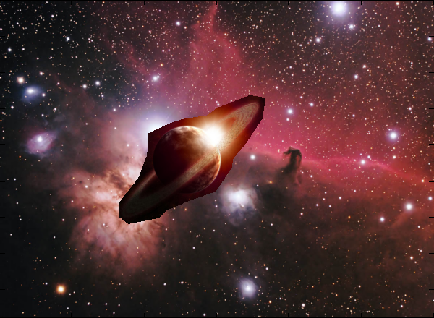
\includegraphics[scale=0.54]{results_poisson/set4/im4.png} 
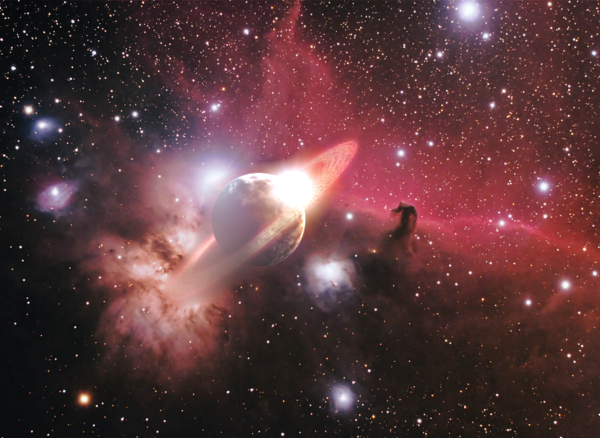
\includegraphics[scale=0.39]{results_poisson/set4/im5.png}   
\caption{My favorite blending result. (left, top) Source object, (right, top) background image,   (left, bottom) cut and paste result, (right, bottom) Poisson blending final result.}
\label{2}
\end{center}
\end{figure}

\quad


\begin{figure} [ht]
\begin{center}
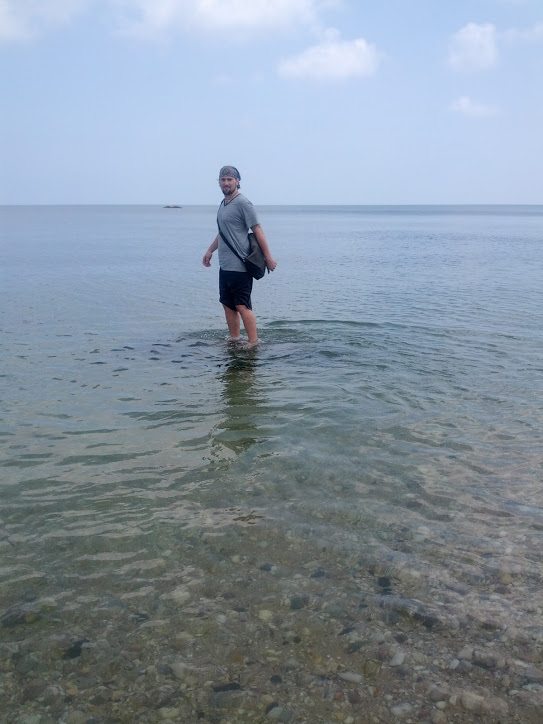
\includegraphics[scale=0.2]{results_poisson/set2/im1.jpg}  
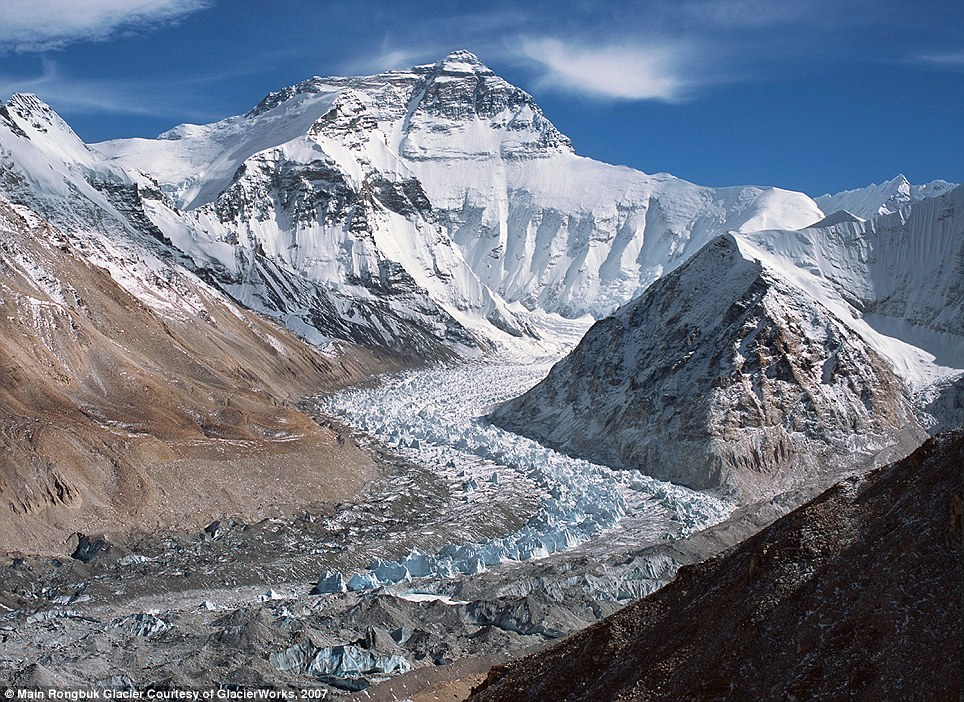
\includegraphics[scale=0.2]{results_poisson/set2/im2.jpg}
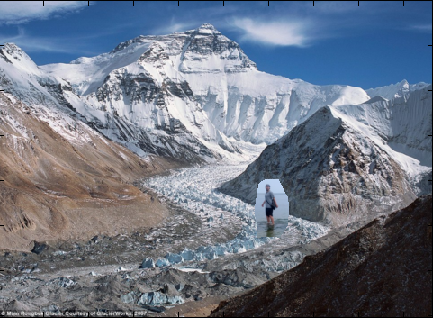
\includegraphics[scale=0.49]{results_poisson/set2/im4.png} 
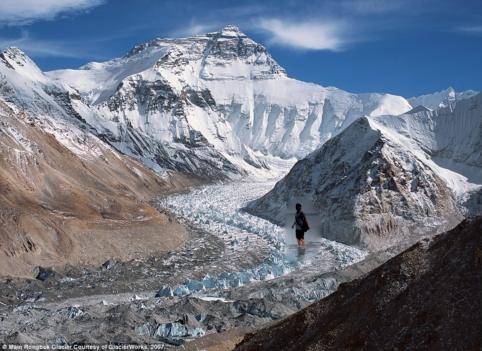
\includegraphics[scale=0.44]{results_poisson/set2/im5.png}   
\caption{An failure example of Poisson example: the texture of the background of the two images are too distant for a simple gradient mixing. (left, top) Source object, (right, top) background image,   (left, bottom) cut and paste result, (right, bottom) Poisson blending final result.}
\label{3}
\end{center}
\end{figure}

\quad






\begin{figure} [ht]
\begin{center}
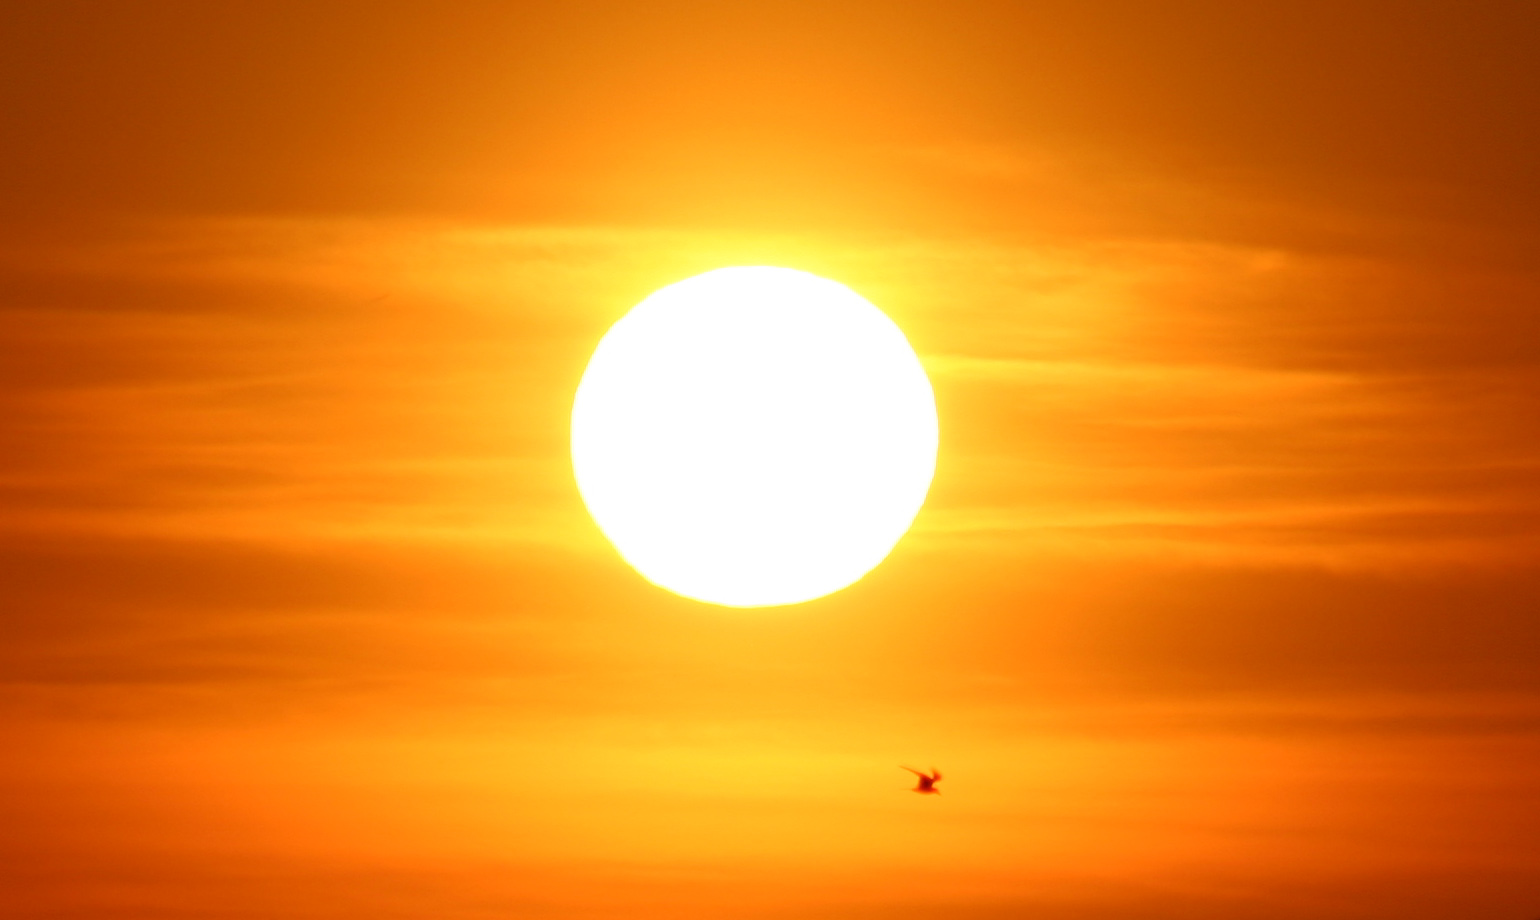
\includegraphics[scale=0.12]{results_poisson/set5/im1.jpg}  
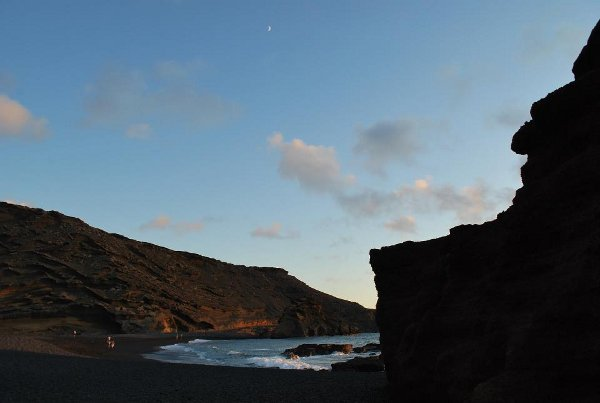
\includegraphics[scale=0.28]{results_poisson/set5/im2.jpg}
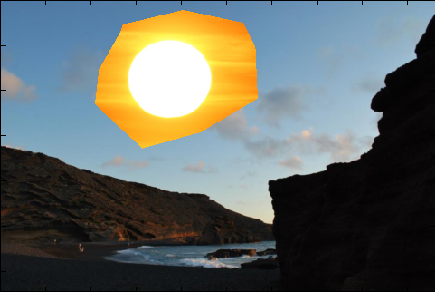
\includegraphics[scale=0.54]{results_poisson/set5/im4.png} 
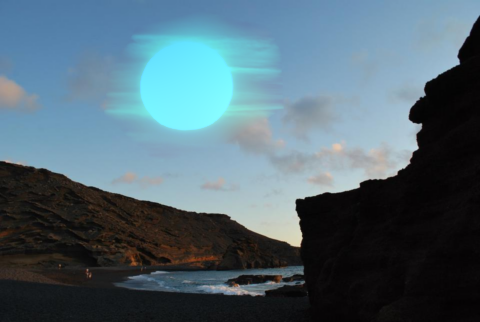
\includegraphics[scale=0.47]{results_poisson/set5/im5.png}   
\caption{Another failure  example of Poisson example, here the gradient literally changes the color of the Sun, however in the object are not corrected.(left, top) Source object, (right, top) background image,   (left, bottom) cut and paste result, (right, bottom) Poisson blending final result.}
\label{4}
\end{center}
\end{figure}

\quad




\subsection*{Mixed Blending}
To improve cases where we see failure in the Poisson bending,  we try to implement an adaptation of the Eq. \ref{aa},
\begin{equation}
v = \mbox{ argmin} \sum_{i \in S, j \in N_i, S} \Bigg ( \Big ( v_i -v_j\Big) - d_{i,j} \Bigg)^2 +  \sum_{i \in S, j \in N_i, -S} \Bigg ( \Big ( v_i -t_j\Big) - d_{i,j} \Bigg)^2,
\end{equation}
where $d_{i,j}$ is the value of the gradient from the source or the target image with {\it larger magnitude}. However this technique  did not show any improvement in the above examples.


\newpage


%%%%%%%%%%%%%%%%%%%%%%%%%%%%%%%%%%%%%%%%%%%%%%%%%%%%%%%%%%%%%%%%%%%%%%%%%%%%%%%%%%%%%%%%%%%%%%
%%%%%%%%%%%%%%%%%%%%%%%%%%%%%%%%%%%%%		Ref		%%%%%%%%%%%%%%%%%%%%%%%%%%%%%%%%%%%%%%%%%%
%%%%%%%%%%%%%%%%%%%%%%%%%%%%%%%%%%%%%%%%%%%%%%%%%%%%%%%%%%%%%%%%%%%%%%%%%%%%%%%%%%%%%%%%%%%%%%



\begin{thebibliography}{}

\bibitem{mike}{\it Tamara Berg's Class}, {\it http://www.tamaraberg.com/teaching/Spring13/compphotog/3}

\bibitem{pois} {\it Poisson Editing}, Patrick Perez, Michel Gangnet, $\&$ Andrew Blacke, 2003

\end{thebibliography}



\end{document}

